\documentclass[AnalisiDeiRequisiti.tex]{subfiles}

\begin{document}

\chapter{Casi d'uso}
\section{Attori dei casi d'uso}
\subsection{Attori primari}
\begin{enumerate}
	\begin{figure}[h]
		\centering
		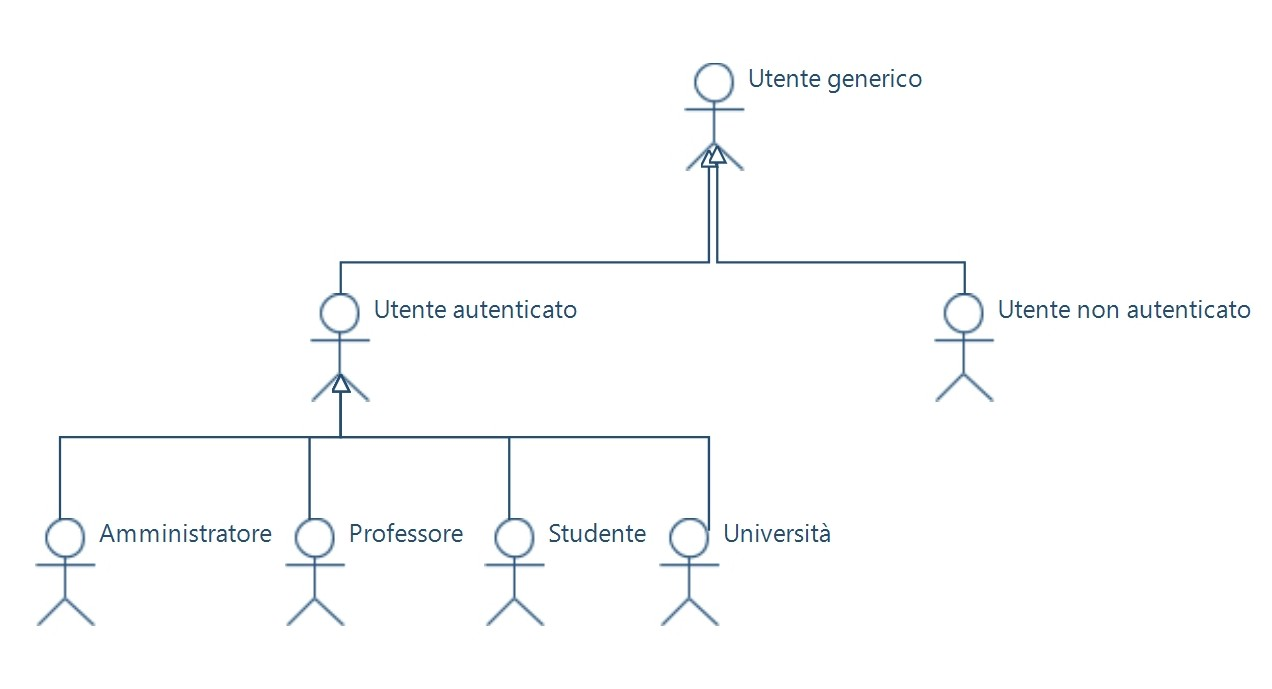
\includegraphics[width=0.6\linewidth]{attoriPrincipali.jpg}
		\caption{Gerarchia attori primari}
		\label{fig:attoriprincipali}
	\end{figure}
	
	\item \textbf{Utente generico}\\
	Si riferisce ad un utente generico che accede al sito\\
	
	\item \textbf{Utente non autenticato}\\
	Ci si riferisce ad un utente generico con non ha ancora effettuato il login.\\
	
	\item \textbf{Utente autenticato}\\
	 Ci si riferisce ad un utente generico con chiave valida ed autenticato nel sistema tramite la procedura di login.\\
	
	\item \textbf{Amministratore}\\
	Ci si riferisce ad un utente autenticato nel sistema nel ruolo di amministratore\\
	
	\item \textbf{Professore}\\
	Ci si riferisce ad un utente autenticato nel sistema nel ruolo di professore.\\
	
	\item \textbf{Studente}\\
	Ci si riferisce ad un utente autenticato nel sistema nel ruolo di studente\\	
\end{enumerate}

\subsection{Attori secondari}
\begin{enumerate}
	\item \textbf{MetaMask}\\
	Plugin del browser MetaMask per interfacciarsi ad una rete Ethereum.\\
	
	\item \textbf{Ufficio immatricolazioni universitario}\\
	Entità fisica che consente l'immatricolazione.\\
\end{enumerate}

\section{Elenco dei casi d'uso}
\subsection{UC1}
\subsection{UC1.1}
\subsection{UC1.2}
\subsection{UC1.2.1}
\subsection{UC2}

\end{document}